\section{Selección de metodología de desarrollo de software}
	\paragraph\indent
	Una metodología indica el camino a seguir para el desarrollo de un proyecto de software. Para el desarrollo del sistema de gestión de la mueblería se utilizará la metodología V-Script.
	\paragraph\indent
	La metodología Script o V-Script es una metodología de desarrollo de software que tiene un alto componente dinámico, orientado hacia la interfaz de usuario. Mediante el proceso Script, se capturan las necesidades del usuario mediante la construcción de maquetas o prototipos desechables, tratando de capturar la expectativa del usuario: qué es lo que el usuario espera que haga el producto.
	\paragraph\indent
	La metodología permite integrar perfectamente los procesos de estimación, gestión de calidad, gestión de configuración y verificación y validación del software. Esta metodología se adapta perfectamente al estándar IEEE 1074-1991: Standard for Developing Software Life Cycle Process.
	\paragraph\indent
	La selección de esta metodología implica que el ciclo de vida mostrado a continuación será el utilizado para completar cada iteración del prototipado evolutivo, recorriendo el modelo una vez por cada iteración. Siendo fundamental la primera iteración para implementar el núcleo.
	\paragraph\indent
		\begin{figure}[H]
            \centering
            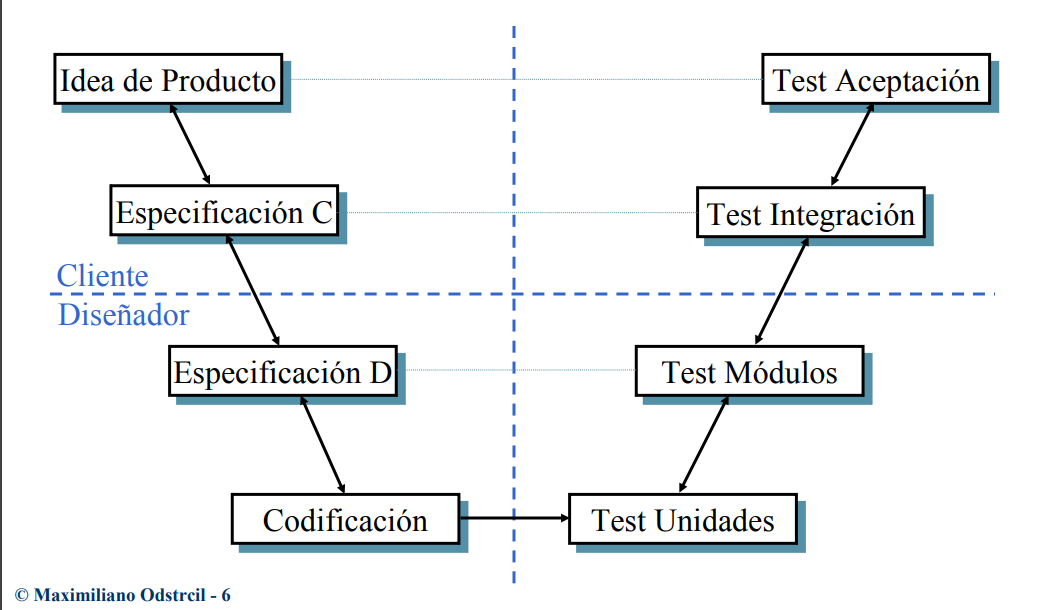
\includegraphics[width=0.8\textwidth,height=0.45\textheight,keepaspectratio]{Extras/DiagramaScript}
            \caption{Diagrama Script}
        \label{fig:diagramaScript}
        \end{figure}
	\paragraph\indent
	En el diagrama puede observarse dos ejes fundamentales:
	\begin{itemize}
		\item \textbf{Eje horizontal}: divide al ciclo de vida en dos partes: una orientada hacia el cliente y otra orientada hacia el desarrollador computadora.
		\item \textbf{Eje vertical}: divide al ciclo de vida en etapas de desarrollo y etapas de prueba del software.
  	\end{itemize}
	Después de finalizada cada etapa, se determina una línea de base. Una línea de base es un punto del ciclo de vida que permite tomar decisiones condicionantes. Se evalúa todo lo realizado hasta ese momento mediante revisiones formales y se decide seguir adelante o bien continuar en cada etapa.
	\paragraph\indent
	Cada etapa Script de desarrollo tiene asociada una etapa de prueba al mismo nivel de abstracción. Estas etapas permiten verificar y validar el producto en los diferentes puntos del camino del producto desde la necesidad hacia la máquina.